\begin{figure}[H]
\begin{subfigure}{.25\textwidth}
  \centering
  \includegraphics[width=.7\linewidth, angle =-90]{img/avg499999stableb.eps}
  \caption{Stable environment.}
  \label{fig:sfig1}
\end{subfigure}%
\begin{subfigure}{.25\textwidth}
  \centering
  \includegraphics[width=.7\linewidth, angle =-90]{img/avg499999variationb.eps}
  \caption{Strong Fluctuation.}
  \label{fig:sfig2}
\end{subfigure}

\begin{subfigure}{.25\textwidth}
  \centering
  \includegraphics[width=.7\linewidth, angle =-90]{img/avg499999variationLightb.eps}
  \caption{Light Fluctuation.}
  \label{fig:sfig2}
\end{subfigure}%
\begin{subfigure}{.25\textwidth}
  \centering
  \includegraphics[width=.7\linewidth, angle =-90]{img/avg499999variationSmallb.eps}
  \caption{Small Fluctuation.}
  \label{fig:sfig1}
\end{subfigure}
\caption{Density of Genotype : Each genotype density is processed in four possible different environments.}
\label{fig:density}
\end{figure}


\subsection{Phenotypic Diversity} 

The phenotypic diversity measured in Figure \ref{fig:phenodiv} can also be observed relatively easily by simple observation of the cellular automaton as it can be seen with a few examples in Figures \ref{fig:phenoexpl}. 



\begin{figure}[H]
\begin{subfigure}{.25\textwidth}
  \centering
  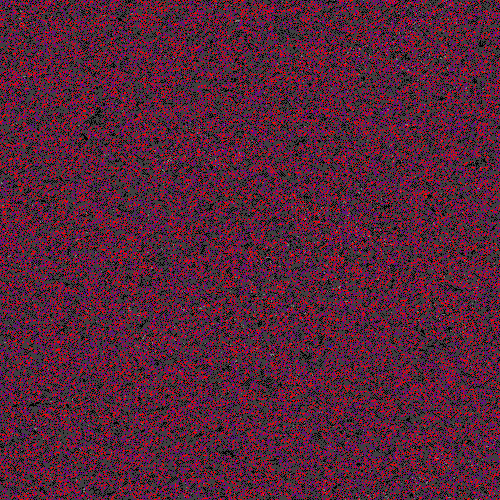
\includegraphics[width=.9\linewidth]{img/stable495000}
  \caption{Stable environment.}
  \label{fig:sfig1}
\end{subfigure}%
\begin{subfigure}{.25\textwidth}
  \centering
  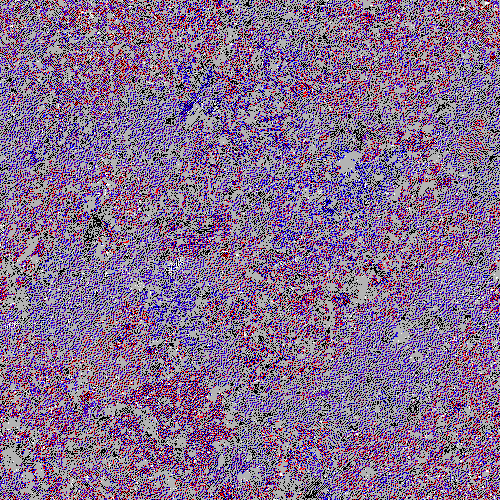
\includegraphics[width=.9\linewidth]{img/var495000}
  \caption{Strong Fluctuation.}
  \label{fig:sfig2}
\end{subfigure}

\begin{subfigure}{.25\textwidth}
  \centering
  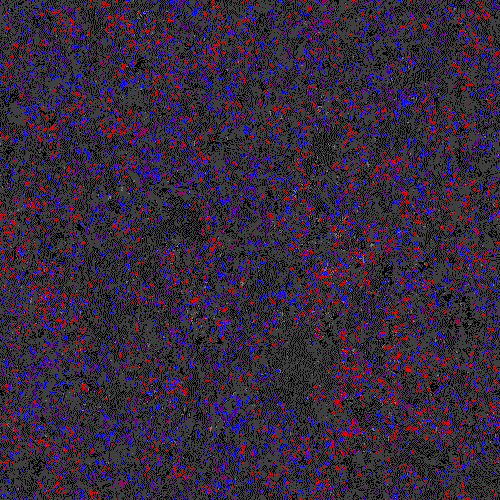
\includegraphics[width=.9\linewidth]{img/light495000}
  \caption{Light Fluctuation.}
  \label{fig:sfig2}
\end{subfigure}%
\begin{subfigure}{.25\textwidth}
  \centering
  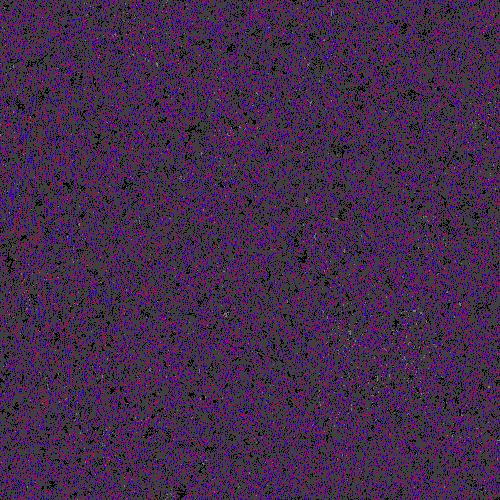
\includegraphics[width=.9\linewidth]{img/small495000}
  \caption{Short-Cycle Fluctuation.}
  \label{fig:sfig1}
\end{subfigure}
\caption{Example of CA gird state repartition (phenotype) at iteration 495000 for the four different configuration. Each cell state is represented by a different color. Black and grey represent respectively cells in \emph{decay} and \emph{quiescent} state.}
\label{fig:phenoexpl}
\end{figure}
